\documentclass[]{article}
\usepackage[a4paper, total={15cm,23cm}]{geometry}
\usepackage{fancyhdr}
\usepackage{graphicx}
\usepackage{amsmath}
\usepackage{amssymb}
\usepackage{xcolor}
\usepackage{tikz}
\usepackage{verbatim}
\usepackage{tcolorbox}
\usepackage{textcomp}
\usepackage{xcomment}
\usepackage{xstring}
\usepackage{array}
%opening
\title{Net Zero Vectors}
\author{Benjamin Bauml}
\date{Winter 2025}
\pagestyle{fancy}
\rhead{PH 221}
\chead{Winter 2025}
\lhead{Week 1}

% Version 2024-02-21
% Changes
% 2024-02-21 Added xstring package to enable smooth implementation of new \ModePage command.
% For Assignment, leave Purpose as 1. For Worksheet, set to 2. For Student Solution, set to 3. For Teacher Solution, set to 4.
\newcommand{\Purpose}{4}

\newcommand{\Exclusion}{0}
\newcommand{\PageTurn}{0}
\newcommand{\GrayProb}{0}
\newcommand{\Tipsy}{0}

% Assignment
\if\Purpose1
\renewcommand{\Exclusion}{1}
\fi
% Worksheet
\if\Purpose2
\renewcommand{\Exclusion}{1}
\renewcommand{\PageTurn}{1}
\fi
% Student Solution
\if\Purpose3
\renewcommand{\PageTurn}{1}
\renewcommand{\GrayProb}{1}
\fi
% Teaching Copy
\if\Purpose4
\renewcommand{\PageTurn}{1}
\renewcommand{\GrayProb}{1}
\renewcommand{\Tipsy}{1}
\fi

\if\Exclusion1
\xcomment{Title,Problem,ProblemSub,PassFig}
\fi

\def \NewQ {0}
\def \PForce {0}
\newcommand{\MaybePage}[1]{
	\def \PForce {#1}
	\if\PForce1
		\newpage
	\else
		\if\NewQ0
		\gdef \NewQ {\PageTurn}
		\else
		\newpage
		\fi
	\fi
}

\newcommand{\ModePage}[1]{
	\IfSubStr{#1}{\Purpose}{\newpage}{}
}

\newenvironment{Problem}[2][0]{%The first argument is optional, and if it is set to 1, the \newpage will be forced.
\MaybePage{#1}
\section*{#2}
\if\GrayProb1
\begin{tcolorbox}[colback=lightgray,colframe=lightgray,sharp corners,boxsep=1pt,left=0pt,right=0pt,top=0pt,bottom=0pt,after skip=2pt]
\else
\begin{tcolorbox}[colback=white,colframe=white,sharp corners,boxsep=1pt,left=0pt,right=0pt,top=0pt,bottom=0pt,after skip=2pt]
\fi
}{
\end{tcolorbox}\noindent
}

\newenvironment{ProblemSub}[1][0]{%The argument is optional, and if a string of numbers is entered into it, it will force a \newpage in any \Purpose that shows up in the string. For example, "13" would lead to the newpage being forced in modes 1 and 3.
\ModePage{#1}
\if\GrayProb1
\begin{tcolorbox}[colback=lightgray,colframe=lightgray,sharp corners,boxsep=1pt,left=0pt,right=0pt,top=0pt,bottom=0pt,after skip=2pt]
\else
\begin{tcolorbox}[colback=white,colframe=white,sharp corners,boxsep=1pt,left=0pt,right=0pt,top=0pt,bottom=0pt,after skip=2pt]
\fi
}{
\end{tcolorbox}\noindent
}

\newenvironment{PassFig}{\begin{figure}[h]}{\end{figure}}

\newcommand{\TeachingTips}[1]{
\if\Tipsy1
\begin{tcolorbox}[colback=lightgray,colframe=black]
#1
\end{tcolorbox}
\fi
}

\newenvironment{Title}{\maketitle}{}

\begin{document}
\begin{Title}
\begin{center}
	This material is borrowed/adapted from the \textit{Learning Introductory Physics with Activities} textbook.
\end{center}
\end{Title}

\begin{Problem}{Activity}
	Three vectors add together to equal 0. One vector has magnitude 3 and points in the positive $x$-direction; a second vector has magnitude 5 and points at 120$^{\circ}$ from the positive $x$-axis. Determine the third vector as a magnitude and direction.
\end{Problem}
Below, I have drawn the two vectors---I'm calling the first vector along the $x$-axis $\vec{a}$, and the angled vector $\vec{b}$. A cyan copy of $\vec{b}$ has been placed at the tip of $\vec{a}$ to illustrate the sum $\vec{a}+\vec{b}$. The red vector is what the third vector needs to be for the three to sum to zero.
\begin{figure}[h]
	\centering
	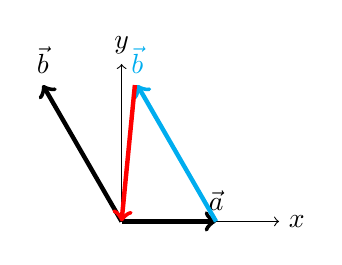
\begin{tikzpicture}
		\draw[<->] (0,2) node[anchor=south] {$y$} -- (0,0) -- (2,0) node[anchor=west] {$x$};
		\draw[->,ultra thick] (0,0) -- (1.2,0) node[anchor=south] {$\vec{a}$};
		\draw[->,ultra thick,rotate=120] (0,0) -- (2,0) node[anchor=south] {$\vec{b}$};
		\draw[->,ultra thick,shift={(1.2,0)},rotate=120,cyan] (0,0) -- (2,0) node[anchor=south] (btip) {$\vec{b}$};
		\draw[->,ultra thick,red] (btip) -- (0,0);
	\end{tikzpicture}
\end{figure}
Based on this representation, we can see that the third vector must be a little shorter than $\vec{b}$, and it will point a little more than 90$^{\circ}$ clockwise from the positive $x$-axis.

Let's break $\vec{b}$ into components:
\[
\begin{split}
	b_{x} & = 5\cos(120^{0}) =-2.5, \\
	b_{y} & = 5\sin(120^{0}) \approx 4.33.
\end{split}
\]
Adding $\vec{a}$ and $\vec{b}$ componentwise gives us
\[
\vec{a}+\vec{b} \approx 3\hat{x} + \left(-2.5\hat{x} + 4.33\hat{y}\right) = 0.5\hat{x} + 4.33\hat{y},
\]
so the third vector (let's call it $\vec{c}$) will be the negative of this:
\[
\vec{c} = -\left(\vec{a}+\vec{b}\right) = -0.5\hat{x} -4.33\hat{y}.
\]
We can get the magnitude via the Pythagorean Theorem:
\[
|\vec{c}| \approx \sqrt{0.5^{2}+4.33^{2}} \approx 4.36.
\]
The angle can be determined trigonometrically, but most calculators will give you the wrong answer first:
\[
\theta^{*} \approx \arctan\left(\frac{-4.33}{-0.5}\right) \approx 83.4.
\]
This would be the angle for $-\vec{c}$. The tangent function has a period of 180$^{\circ}$, so we can subtract this to get another valid angle in the correct quadrant:
\[
\theta = \theta^{*} - 180^{\circ} \approx -96.6^{\circ}.
\]
\end{document}